\usepackage{tikz}

\section*{Problem C - Crewmate dan Impostor}
\textit{Author: Muhammad Fahmi Irfan, Ahmad Romy Zahran}
\\
\textit{Expected Difficulty: Medium}

Perhatikan representasi graf berarah, setiap komponen memiliki banyak \textit{node} sama dengan banyak \textit{edge}. Akibatnya, setiap komponen merupakan graf dengan 1 \textit{cycle}. 

Perhitungan banyak impostor maksimal pada setiap komponen dapat dilakukan dengan \textit{dynamic programming}. Pada setiap \textit{node} disimpan informasi banyak \textit{impostor} maksimal untuk \textit{subtree} tersebut bila \textit{node} tersebut \textit{crewmate} ($dp[0]$) dan bila \textit{node} tersebut \textit{impostor} ($dp[1]$). Untuk bagian \textit{tree}, berlaku persamaan berikut:

$$ dp_u[0] = \sum_{v \in children_u} max(dp_v[0],dp_v[1]) $$
$$ dp_u[1] = 1 + \sum_{v \in children_u} dp_v[0] $$

\begin{center}
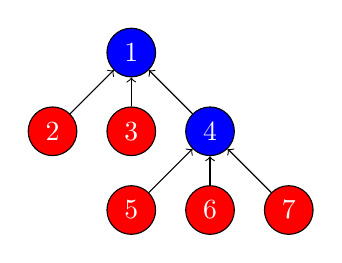
\begin{tikzpicture}
[impostor/.style = {draw, circle, fill=red, font=\color{white}, scale=1}, 
crewmate/.style = {draw,circle, fill=blue, font=\color{white}, scale=1}] 
\node[crewmate] (1) {$1$}; 
\node[impostor] (3) [below of =1]{$3$};
\node[impostor] (2) [left of =3]{$2$}; 
\node[crewmate] (4) [right of =3] {$4$}; 
\node[impostor] (6) [below of =4]{$6$};
\node[impostor] (5) [left of =6]{$5$}; 
\node[impostor] (7) [right of =6]{$7$};
\draw[->] (2)--(1);
\draw[->] (3)--(1);
\draw[->] (4)--(1);
\draw[->] (5)--(4);
\draw[->] (6)--(4);
\draw[->] (7)--(4);
\end{tikzpicture}
\end{center}

Perhitungan bagian \textit{tree} dilakukan seperti \textit{topologycal sort} melalui \textit{in degree}. Untuk bagian \textit{cycle}, setiap \textit{cycle} disimpan informasi maximal \textit{impostor} sesuai kemungkinan ujung kiri dan kanannya.

\begin{center}
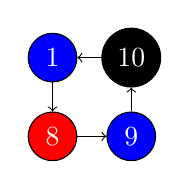
\begin{tikzpicture}
[impostor/.style = {draw, circle, fill=red, font=\color{white}, scale=1}, 
crewmate/.style = {draw,circle, fill=blue, font=\color{white}, scale=1},
unknown/.style = {draw,circle,fill=black, font=\color{white}, scale=1}] 
\node[crewmate] (1) {$1$}; 
\node[impostor] (2) [below of =1]{$8$}; 
\node[crewmate] (3) [right of =2]{$9$};
\node[unknown] (4) [right of =1] {$10$}; 
\draw[->] (1)--(2);
\draw[->] (2)--(3);
\draw[->] (3)--(4);
\draw[->] (4)--(1);
\end{tikzpicture}
\end{center}

Jawaban yang diinginkan adalah penjumlahan dari maximal \textit{impostor} di setiap komponen, kemudian dibandingkan dengan $\lfloor \frac{n-1}{2} \rfloor$ dan diambil yang minimal.

Kode Solusi: \url{https://ideone.com/D294XE}

Kompleksitas Waktu: $O(n)$